\chapter{Conceitos}

Este cap�tulo apresentar� a forma como os conceitos presentes no trabalho se interligaram, mostrando o sistema proposto, suas principais caracter�sticas, componentes e funcionalidades.

\section{Sistema}

\begin{listagem}
\begin{verbatim}
 Aqui vai o algor�tmo...
\end{verbatim}
\caption{Este algor�tmo faz o seguinte...}
\end{listagem}


\subsection{Descri��o}

Prop�e-se o desenvolvimento de um prot�tipo de um sistema de buscas por m�sicas baseado em conte�do, este sistema recebe uma entrada do usu�rio que corresponde � sua \query, ou seja, algum trecho da m�sica buscada que o usu�rio reproduza atrav�s de um assobio. O sistema recebe a \query \ e em seguida compara com as m�sicas presentes em seu reposit�rio, calculando a similaridade entre cada m�sica e a \query, a partir das compara��es efetuadas, o sistema � capaz de apresentar quais as entradas mais prov�veis de corresponderem � m�sica procurada.

\subsubsection{Espa�o de busca}

O espa�o de busca ser� constitu�do por m�sicas em formato MIDI, devidamente preparadas para o ambiente de execu��o de buscas. Pelo fato dos arquivos MIDI, na maioria dos casos, possuirem diversas trilhas, devem portanto passar por um processo de prepara��o, onde apenas a trilha mais relevante da m�sica � extra�da e ent�o adicionada ao reposit�rio. Devido ao foco dado ao sistema este processo se desenvolveu manualmente, atrav�s de uma an�lise humana de cada trilha, escolhendo a mais relevante.


\subsubsection{Entrada de dados}

A entrada do sistema dar� origem 





\begin{figure}[htb]
	\center{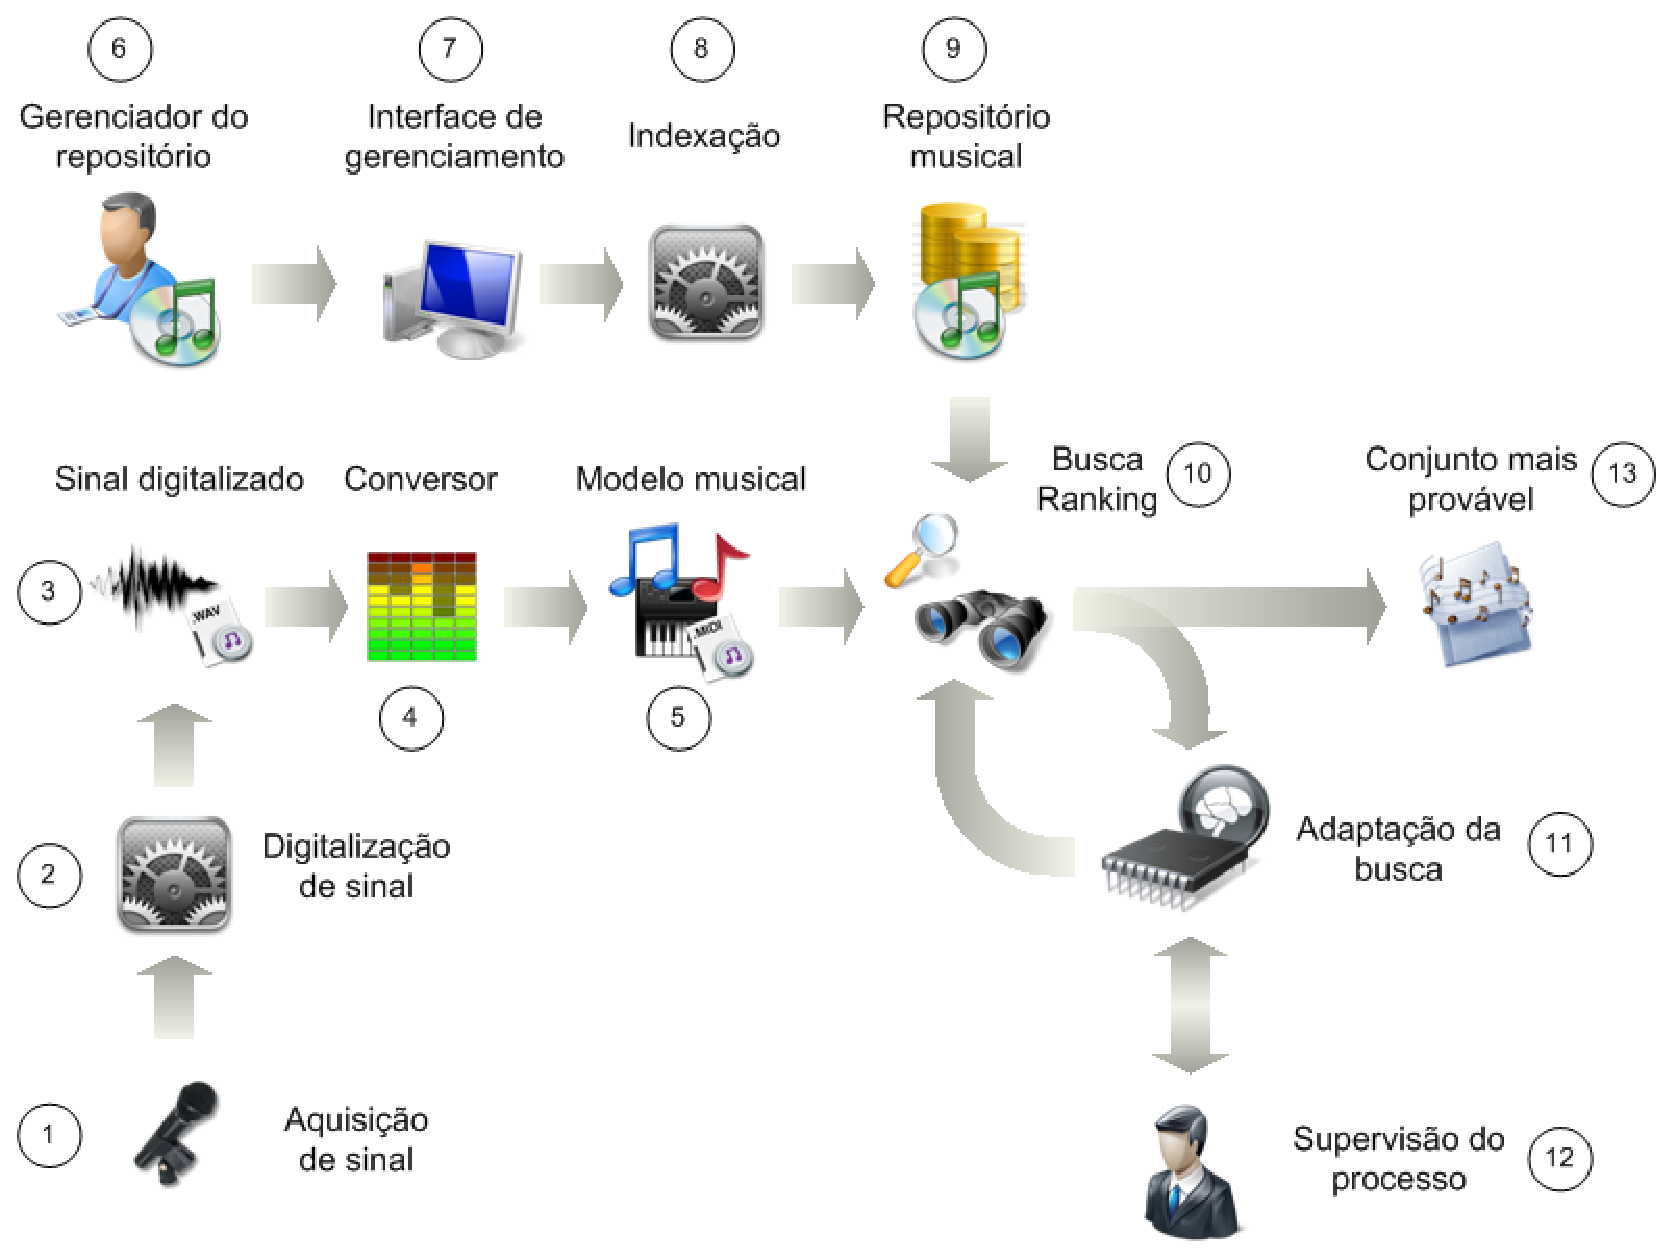
\includegraphics[width=0.85\textwidth]{figuras/arquitetura.eps}}
	\caption{\label{fig:arquitetura} Arquitetura do sistema}
\end{figure}

\section{Processamento de sinais}

\section{Adaptatividade}